\begin{center}
    \textsc{\large\textbf{Illustrations: Slope, Line}}
\end{center}
\BgThispage
\begin{enumerate}
    \item Find the slope and also write the equation of the given straight lines:
        \begin{tasks}(2)
            \task 
                \begin{center}
                    \begin{tikzpicture}[scale=0.75]
                        \tzaxes(-1, -2)(4, 2){$x$}{$y$}
                        \tzcoors*(2, 1)(B){$(2,1)$}[al](0, -1)(A){$(0, -1)$}[l];
                        \tzLFn(A)(B)[-1:2.5]
                    \end{tikzpicture}
                \end{center}

            \task
                \begin{center}
                    \begin{tikzpicture}[scale=0.75]
                        \tzaxes(-1, -1)(4, 3){$x$}{$y$}
                        \tzcoors*(0, 2)(A)(2, 0)(B){$2$}[bl];
                        \tzLFn(A)(B)[-1:3]
                        \tzanglemark(3, 0)(B)(A){$135^\circ$}[pos=2.5]
                    \end{tikzpicture}
                \end{center}

            \task 
            \begin{center}
                \begin{tikzpicture}[scale=0.75]
                    \tzaxes(-1, -1.5)(4, 3){$x$}{$y$}
                    \tzcoors*(0, 2)(A)(1.5, 0)(B){$1$}[bl];
                    \tzLFn(A)(B)[-0.8:2.75]
                    \tzanglemark'(B)(A)(0, 3){$150^\circ$}[pos=2.5]
                \end{tikzpicture}
            \end{center}

            \task 
                \begin{center}
                    \begin{tikzpicture}[scale=0.75]
                        \tzaxes(-1, -1)(4, 3){$x$}{$y$}
                        \tzcoors*(0, 0)(A)(2.5, 1.5)(B){$(3, \sqrt{3})$}[al];
                        \tzLFn(A)(B)[-1:3]
                    \end{tikzpicture}
                \end{center}
            
            \task 
                \begin{center}
                    \begin{tikzpicture}[scale=0.75]
                        \tzaxes(-3, -1)(3, 3){$x$}{$y$}
                        \tzcoors*(-2, 0)(A){$-2$}[b](0, 1)(B){$1$}[al];
                        \tzLFn(A)(B)[-3:2.5]
                    \end{tikzpicture}
                \end{center}

            \task
                \begin{center}
                    \begin{tikzpicture}[scale=0.75]
                        \tzaxes(-1, -1)(4, 3){$x$}{$y$}
                        \tzcoors*(0, 2)(A){$2$}[al](2, 2)(B){$(2, 2)$}[ar];
                        \tzLFn(A)(B)[-1:3]
                        \tzline[dashed] (2, 0)(2, 3)
                    \end{tikzpicture}
                \end{center}

            \task
                \begin{center}
                    \begin{tikzpicture}[scale=0.75]
                        \tzaxes(-1, -1)(4, 3){$x$}{$y$}
                        \tzcoors*(2, 0)(B){$2$}[br];
                        \tzline(2, -1)(2, 2.5)
                        \tzrectangle(2, 0)(2.4, 0.4)
                    \end{tikzpicture}
                \end{center}

            \task
                \begin{center}
                    \begin{tikzpicture}[scale=0.75]
                        \tzaxes(-1, -1)(4, 3){$x$}{$y$}
                        \tzcoors*(0, 0)(A);
                        \tzline(0, 0)(3, 3)
                        \tzanglemark(3, 0)(0, 0)(3, 3){$45^\circ$}[pos=2.5]
                    \end{tikzpicture}
                \end{center}
        \end{tasks}
        
        \begin{solution}
           
            \begin{enumerate}
                \item 
                    \begin{align*}
                        \intertext{We can use the two-point form to find the slope of the line. Slope:}
                        m &= \frac{y_2-y_1}{x_2-x_1} = \frac{1-(-1)}{2-0} = 1
                        \intertext{For the equation of the line, we can use the slope-intercept form. Equation:}
                        y &= mx + c \\
                        y &= x - 1
                    \end{align*}

                \item
                    \begin{align*}
                        \intertext{We can use $\tan\theta$ as the $\theta$ is known here. Slope:}
                        m &= \tan 135^\circ = \tan (180^\circ - 45^\circ) = -\tan 45^\circ = -1
                        \intertext{For the equation of the line, we can use the slope-point form. Equation:}
                        y - y_1 &= m(x - x_1) \\
                        y - 0 &= -1(x - 2) \\
                        y &= -x + 2
                    \end{align*}

                \item
                \begin{multicols}{2}
                    \begin{align*}
                        \intertext{We can use $\tan\theta$ as the $\theta$ is known here. Slope:}
                        m &= \tan 120^\circ \\
                        &= \tan (180^\circ - 60^\circ) \\
                        &= -\tan 60^\circ \\
                        &= -\sqrt{3}
                        \intertext{For the equation of the line, we can use the slope-point form. Equation:}
                        y - y_1 &= m(x - x_1) \\
                        y - 0 &= -\sqrt{3}(x - 1) \\
                        y &= -\sqrt{3}x + \sqrt{3}
                    \end{align*}
                    \begin{center}
                        \begin{tikzpicture}[scale=0.75]
                            \tzaxes(-1, -1.5)(4, 4){$x$}{$y$}
                            \tzcoors*(0, 2)(A)(1.5, 0)(B){$1$}[bl];
                            \tzLFn(A)(B)[-0.8:2.75]
                            \tzanglemark'(B)(A)(0, 3){$150^\circ$}[pos=2.5]
                            \tzanglemark(0, 0)(A)(B){$30^\circ$}[pos=2](15pt)
                            \tzanglemark(A)(B)(0, 0){$60^\circ$}[pos=2]
                            \tzanglemark(4, 0)(B)(A){$120^\circ$}[pos=2](12pt)
                        \end{tikzpicture}
                    \end{center}
                \end{multicols}
                \BgThispage
                \item
                    \begin{align*}
                        \intertext{We can use the two-point form to find the slope of the line. Slope:}
                        m &= \frac{y_2-y_1}{x_2-x_1} = \frac{\sqrt{3}-0}{3-0} = \frac{1}{\sqrt{3}}
                        \intertext{For the equation of the line, we can use the slope-intercept form. Equation:}
                        y &= mx + c \\
                        y &= \frac{1}{\sqrt{3}}x
                    \end{align*}

                \item
                    \begin{align*}
                        \intertext{We can use $\tan\theta$ in the triangle formed by line and both axes. Slope:}
                        m &= \tan \theta = \frac{1}{2}
                        \intertext{For the equation of the line, we can use the slope-intercept form. Equation:}
                        y &= mx + c \\
                        y &= \frac{1}{2}x + 1
                    \end{align*}

                \item
                    \begin{align*}
                        \intertext{Line is horizontal, slope is zero.}
                        m &= 0
                        \intertext{For the equation of the line, we can use the slope-intercept form. Equation:}
                        y &= mx + c \\
                        y &= 2
                    \end{align*}

                \item
                    \begin{align*}
                        \intertext{Line is vertical, slope is undefined.}
                        m &= \text{undefined}
                        \intertext{For the equation of the line, we can observe that for every value of $y$, $x$ remains $2$. Equation:}
                        x &= 2\\[5mm]
                        \intertext{or, we can use the intercept form. Equation:}
                        \frac{x}{a} + \frac{y}{b} &= 1 \\
                        \intertext{$a=2$, $b \to \infty/-\infty$}
                        \frac{x}{2} &= 1\\
                        x &= 2
                    \end{align*}

                \item
                    \begin{align*}
                        \intertext{We can use $\tan\theta$. Slope:}
                        m &= \tan \theta = \tan 45^\circ = 1
                        \intertext{For the equation of the line, we can use the slope-intercept form. Equation:}
                        y &= mx + c \\
                        y &= x
                    \end{align*}
            \end{enumerate}
            \BgThispage
        \end{solution}

    \item Find the point of intersection of lines $y=x+4 \quad \text{and} \quad y=2x$. Also, find the equation of the line passing through their point of intersection and having slope $-1$.
        \begin{solution}
            \begin{align*}
                y &= x + 4 \\
                y &= 2x \\
                \intertext{Equating the two equations,}
                x + 4 &= 2x \\
                x &= 4 \\
                \intertext{Substituting the value of $x$ in the second equation,}
                y &= 2(4) = 8 \\
                \intertext{The point of intersection is $(4, 8)$.}
                \intertext{The equation of the line passing through the point of intersection and having slope $-1$ is}
                y - y_1 &= m(x - x_1) \\
                y - 8 &= -1(x - 4) \\
                y - 8 &= -x + 4 \\
                y &= -x + 12
            \end{align*}
        \end{solution}

    
    \item Find the angle between the straight lines $x-y=0$ and $x+y=0$.
        \begin{solution}
            \begin{align*}
                x - y &= 0 \\
                y &= x \\
                m_1 &= 1 \tag{1}\\
                x + y &= 0 \\
                y &= -x \\
                m_2 &= -1 \tag{2}
                \intertext{The angle between two lines is given by}
                \tan \theta &= \left| \frac{m_2 - m_1}{1 + m_1m_2} \right| \\
                \tan \theta &= \left| \frac{-1 - 1}{1 + 1(-1)} \right| \\
                \tan \theta &= \left| \frac{-2}{0} \right| \\
                \tan \theta &\to \infty \\
                \theta &= 90^\circ
            \end{align*}        
        \end{solution}
        \BgThispage
    \item Find the equation of the straight line passing through $(2, 3)$ and perpendicular to the straight line passing through $(-1, 0)$ and (3, 8).
        \begin{solution}
            \begin{align*}
                \intertext{The slope of the line passing through $(-1, 0)$ and $(3, 8)$ is}
                m &= \frac{8-0}{3-(-1)} = \frac{8}{4} = 2
                \intertext{The slope of the line perpendicular to this line is}
                m &= -\frac{1}{2}
                \intertext{The equation of the line passing through $(2, 3)$ and having slope $-\frac{1}{2}$ is}
                y - y_1 &= m(x - x_1) \\
                y - 3 &= -\frac{1}{2}(x - 2) \\
                y - 3 &= -\frac{1}{2}x + 1 \\
                y &= -\frac{1}{2}x + 4
            \end{align*}
        \end{solution}
\end{enumerate}


